
\chapter{Statistical results}


\begin{figure}[H]
  \centering
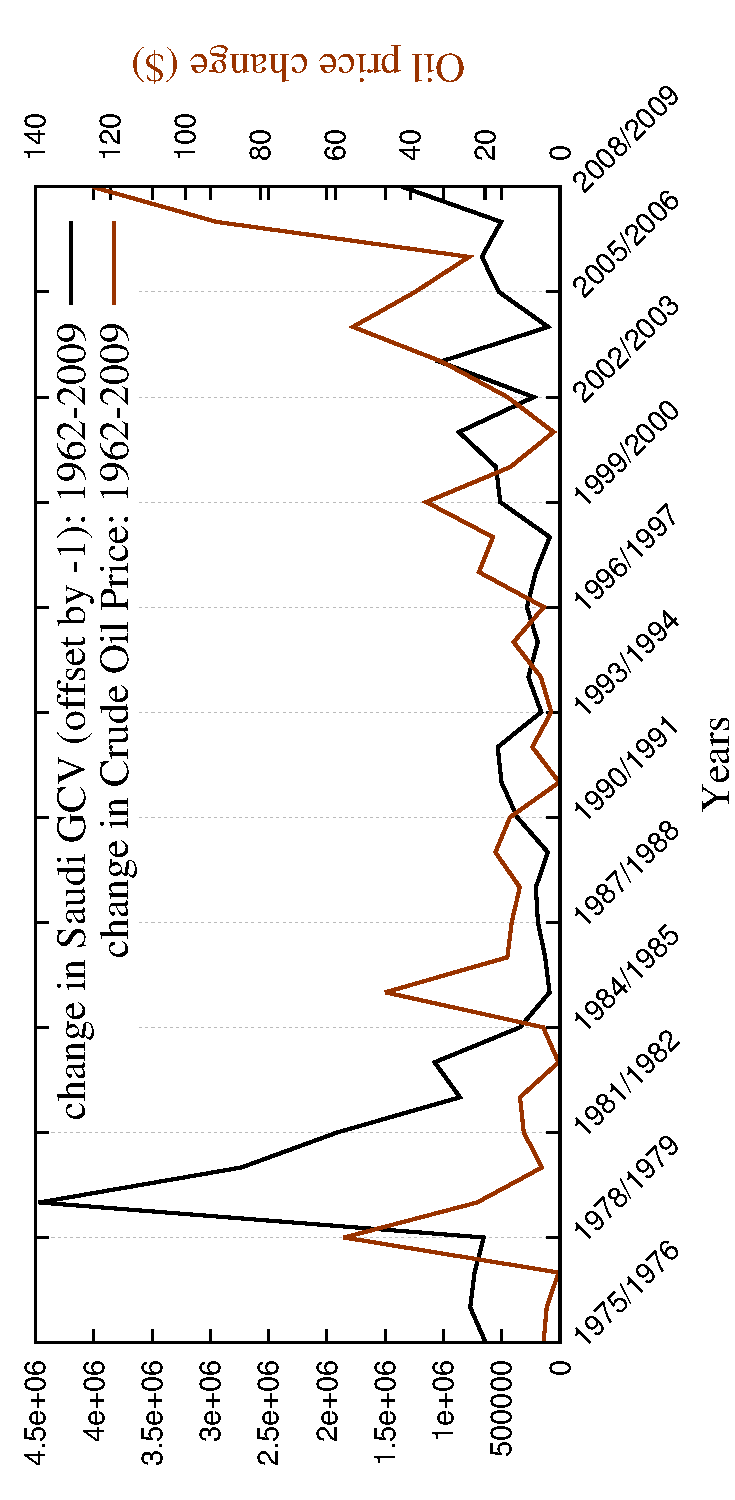
\includegraphics[angle=-90,scale=0.6]
{../code/extra_results/saudi_oil/saudi_orig_gcv_oil2}
\caption[The change in the un-normalised GCV of Saudi Arabia along with the change in Crude Oil price.]{The change in the un-normalised GCV of Saudi Arabia along with the change in Crude Oil price. The un-normalised GCV is not suitable for correlating the GCV of Saudi Arabia with the change in crude oil price, because Spearman's rank correlation coefficient is small (less than 0.13), while the p-value is large (bigger than 0.35). This is the case for all shifts in GCV in the range $[-2,2]$}
\label{saudi_oil_orig}
\end{figure}

\chapter{Canonical Correlation Tables}


\definecolor{col1}{HTML}{5752FF} % blue
\definecolor{col2}{HTML}{05D1FF} % 
\definecolor{col3}{HTML}{85FFA3} % 
\definecolor{col4}{HTML}{C8FF85} % 
\definecolor{col5}{HTML}{F5FF85} % 
\definecolor{col6}{HTML}{FFA985} % 
\definecolor{col7}{HTML}{FF8585} % red



\begin{figure}[H]
  \begin{subfigure}{.7\textwidth}
  \centering
  \begin{tabular}{ c c | c c }
    \multicolumn{2}{c}{Canonical Correlation} &  \multicolumn{2}{c}{0.89595} \\
    \multicolumn{2}{c}{p-value} &  \multicolumn{2}{c}{0.00000} \\
    \hline
    \multicolumn{2}{c}{X variate} & \multicolumn{2}{c}{Y variate}\\
    \hline
  POP & 0.76667 &  G1 & 0.82332\\
  LE & 0.75818 &  G2 & 0.80569\\
  KIxRGDPLxPOP & 0.72552 &  G6 & 0.80315\\
  RGDPCHxPOP & 0.71889 &  G7 & 0.79365\\
  RGDPLxPOP & 0.71877 &  G3 & 0.78361\\
  RGDPL2xPOP & 0.71683 &  G4 & 0.78270\\
  KCxRGDPLxPOP & 0.69962 &  G17 & 0.77813\\
  KGxRGDPLxPOP & 0.69344 &  G22 & 0.76781\\
  KCxRGDPL & 0.42077 &  G23 & 0.76656\\
  RGDPCH & 0.26634 &  G24 & 0.76458\\
  RGDPL & 0.26629 &  G14 & 0.76293\\
  RGDPL2 & 0.26616 &  G26 & 0.75734\\
  KGxRGDPL & 0.21884 &  G8 & 0.75020\\
  KIxRGDPL & 0.17869 &  G13 & 0.74857\\
  XRAT & 0.11999 &  G19 & 0.74581\\
  KC & 0.09780 &  G28 & 0.74525\\
  KI & -0.05999 &  G18 & 0.74056\\
  BCAperRGDPL & -0.14775 &  G12 & 0.74053\\
  KG & -0.17422 &  G11 & 0.73369\\
  BCA & -0.20019 &  G10 & 0.72915\\
  OPENK & -0.24745 &  G9 & 0.72424\\
  & &  G27 & 0.70899\\
  & &  G29 & 0.68727\\
  & &  G21 & 0.67142\\
  & &  G5 & 0.66142\\
  & &  G25 & 0.63754\\
  & &  G16 & 0.62203\\
  & &  G15 & 0.57546\\
  & &  G20 & 0.44454\\
  \end{tabular}
  \end{subfigure}
  \begin{subfigure}{.25\textwidth}
    \centering 
    \rowcolors{1}{}{}		
    
    \gone
    \gtwo
    \gsix
    \gdots
    \gsixteen
    \gfifteen
    \gtwenty
    
  \end{subfigure}
  
  \caption[CCA - World Trade Network - unnormalised GCV]{Canonical Correlation Analysis between economic indicators ($X$ variate) and the unnormalised GCV signature ($Y$ variate) on the 2010 World Trade network. Openness (OPENK), Balance Current Account (BCA) a few other indicators correlate negatively with all the graphlets, because their cross-loadings have different signs. On the other hand, the rest of the indicators such as Population (POP), Level of Employment (LE) and GDP per capita (RGPDL, RGDPCH) correlate positively with all the graphlets, since their cross-loadings have the same sign. The overall correlation is 0.89 with a p-value of 0.0. In reality, the p-value is extremely small but it has been truncated to zero because of floating point approximations.}
  \label{all_trade_thresh_cca_orig}
\end{figure}




\begin{figure}[H]
  \begin{subfigure}{.65\textwidth}
  \centering
  \begin{tabular}{ c c | c c }
    \multicolumn{2}{c}{Canonical Correlation} &  \multicolumn{2}{c}{0.94594} \\
    \multicolumn{2}{c}{p-value} &  \multicolumn{2}{c}{0.00000} \\
    \hline
    \multicolumn{2}{c}{X variate} & \multicolumn{2}{c}{Y variate}\\
    \hline
  POP & 0.73628 &  \cellcolor{col2} G12 & 0.90456\\
  LE & 0.71650 &  \cellcolor{col1} G10 & 0.89337\\
  KI x RGDPL x POP & 0.66038 &  \cellcolor{col2}G14 & 0.87536\\
  RGDPCH x POP & 0.65383 &  \cellcolor{col3}G17 & 0.85955\\
  RGDPL x POP & 0.65376 &  \cellcolor{col1}G9 & 0.84692\\
  RGDPL2 x POP & 0.65226 &  \cellcolor{col1}G11 & 0.83708\\
  KG x RGDPL x POP & 0.64238 &  \cellcolor{col3}G19 & 0.70966\\
  KC x RGDPL x POP & 0.63303 &  \cellcolor{col1}G4 & 0.69198\\
  KC x RGDPL & 0.29252 &  \cellcolor{col2}G16 & 0.67490\\
  XRAT & 0.17083 &  \cellcolor{col1}G3 & 0.63019\\
  RGDPCH & 0.16079 &  \cellcolor{col3}G18 & 0.60564\\
  RGDPL & 0.16071 &  \cellcolor{col4}G24 & 0.59760\\
  RGDPL2 & 0.16038 &  \cellcolor{col2}G13 & 0.59247\\
  KG x RGDPL & 0.15848 &  \cellcolor{col4}G22 & 0.54531\\
  KI x RGDPL & 0.10411 &  \cellcolor{col4}G23 & 0.47154\\
  KC & 0.08634 &  \cellcolor{col2}G15 & 0.43876\\
  KI & -0.01620 &  \cellcolor{col3}G21 & 0.32221\\
  BCA per RGDPL & -0.10953 &  \cellcolor{col3}G20 & 0.28966\\
  KG & -0.12868 &  \cellcolor{col5}G26 & 0.27068\\
  BCA & -0.14935 &  \cellcolor{col3}G6 & 0.23057\\
  OPENK & -0.26502 &  \cellcolor{col5}G27 & 0.15386\\
  & &  \cellcolor{col4}G25 & 0.14823\\
  & &  \cellcolor{col3}G5 & 0.11232\\
  & &  \cellcolor{col6}G28 & -0.15016\\
  & &  \cellcolor{col5}G1 & -0.16367\\
  & &  \cellcolor{col6}G7 & -0.21277\\
  & &  \cellcolor{col7}G2 & -0.48656\\
  & &  \cellcolor{col7}G29 & -0.52462\\
  & &  \cellcolor{col7}G8 & -0.63741\\
  \end{tabular}

  \end{subfigure}
  \begin{subfigure}{.25\textwidth}
    \centering 
    \rowcolors{1}{}{}		
	
    \gtwelve
    \gten
    \gfourteen
    \gdots
    \gtwo
    \gtwentynine
    \geight

  \end{subfigure}
  
\caption[CCA - World Trade networks - normalised GCV]{CCA between the economic indicators and the normalised GCV signature on the 2010 World Trade network. Each graphlet has been colour-coded according to its density, from sparse graphlets in blue to dense graphlets and cliques in red. One can notice how the sparse graphlets have a positive cross-loading, while the dense graphlets have a negative cross-loading. Sparse graphlets are correlated with good economic indicators such as Population (POP), Level of Employment (LE) and GDP per Capita (RGDPL), while dense graphlets are correlated with bad indicators such as the Balance of Current Account (BCA).\hilight{Add a bar showing what the colours mean}}
\label{all_trade_thresh_cca}
\end{figure}


\begin{figure}
  \begin{subfigure}{.65\textwidth}
  \centering
  \begin{tabular}{ c c | c c }
    \multicolumn{2}{c}{Canonical Correlation} &  \multicolumn{2}{c}{0.53013} \\
    \multicolumn{2}{c}{p-value} &  \multicolumn{2}{c}{0.00000} \\
    \hline
    \multicolumn{2}{c}{X variate} & \multicolumn{2}{c}{Y variate}\\
    \hline
  Ribosome translation & 0.91618 &  G2 & 0.89916\\
  RNA processing & 0.08561 &  G8 & 0.86246\\
  Protein degredation  & -0.01381 &  G29 & 0.83575\\
  Cell cycle & -0.01819 &  G7 & 0.81776\\
  Nuclear cytoplasmic transport & -0.07635 &  G1 & 0.81549\\
  ER Golgi traffic & -0.10132 &  G28 & 0.79973\\
  Protein folding & -0.10205 &  G26 & 0.76710\\
  Chromatin  segmentation & -0.12005 &  G27 & 0.75955\\
  Signaling stress response & -0.12897 &  G5 & 0.74980\\
  Cell polarity morphogenesis & -0.14394 &  G6 & 0.73719\\
  Chromatin transcription & -0.14560 &  G22 & 0.72618\\
  DNA replication & -0.17095 &  G24 & 0.71387\\
  Metabolism mitochondria & -0.17109 &  G25 & 0.70796\\
  Golgi endosome vacuole sorting & -0.20098 &  G23 & 0.67823\\
  & &  G4 & 0.65612\\
  & &  G20 & 0.65406\\
  & &  G17 & 0.63899\\
  & &  G21 & 0.61750\\
  & &  G19 & 0.59378\\
  & &  G3 & 0.59369\\
  & &  G16 & 0.54884\\
  & &  G14 & 0.54406\\
  & &  G18 & 0.53288\\
  & &  G15 & 0.52898\\
  & &  G12 & 0.52683\\
  & &  G11 & 0.49169\\
  & &  G13 & 0.41908\\
  & &  G10 & 0.41706\\
  & &  G9 & 0.38194\\

  \end{tabular}

  \end{subfigure}
  \begin{subfigure}{.25\textwidth}
    \centering 
    \rowcolors{1}{}{}		
	
	
    \gtwo
    \geight
    \gtwentynine
    \gdots
    \gthirteen
    \gten
    \gnine
    
    
    


  \end{subfigure}
  
\caption[CCA Analysis on Collin's AP-MS Yeast PPI network.]{CCA Analysis on Collin's AP-MS Yeast PPI network. The $X$ variate is represented by Boone's protein annotations (see section \ref{ppi_annotations}), while the $Y$ variate is represented by the GCV signature. The correlation value is 0.53 and the p-value is shown as 0.0 due to floating point approximations, although in reality it is very low but not exactly 0.0. RNA processing and Ribosome translation correlate positively with all the graphlets because their weights have the same sign, while the rest of the protein annotations correlate negatively with all the graphlets.}
\label{yeast_apms_collins_cca}
\end{figure}


\section{The 17 experiments}

In this section we only show the results that were statistically significant. All the other results can be found in the source code under \lstinline|final_results/all_ppi/|


% ./6-yeast_apms_collins_boone_CCA/CCA_out/yeast_apms_collins.txt

% \begin{figure}[H]
% \centering
% \begin{tabular}{ c c | c c }
%   \multicolumn{2}{c}{Canonical Correlation} &  \multicolumn{2}{c}{0.53013} \\
%   \multicolumn{2}{c}{p-value} &  \multicolumn{2}{c}{0.00000} \\
%   \hline
%   \multicolumn{2}{c}{X variate} & \multicolumn{2}{c}{Y variate}\\
%   \hline
%  Golgi endosome vacuole sorting & 0.11166 &  G9 & -0.21219\\
%  Metabolism mitochondria & 0.09505 &  G10 & -0.23170\\
%  DNA replication   repair HR cohesion & 0.09497 &  G13 & -0.23282\\
%  Chromatin transcription & 0.08089 &  G11 & -0.27316\\
%  Cell polarity morphogenesis & 0.07997 &  G12 & -0.29269\\
%  Signaling stress response & 0.07165 &  G15 & -0.29388\\
%  Chrom  seg  kinetoch  spindle microtub  & 0.06670 &  G18 & -0.29605\\
%  Protein folding   glycosylation cell wall & 0.05669 &  G14 & -0.30226\\
%  ER Golgi traffic & 0.05629 &  G16 & -0.30491\\
%  Nuclear cytoplasmic transport & 0.04242 &  G3 & -0.32983\\
%  Cell cycle progression meiosis & 0.01010 &  G19 & -0.32988\\
%  Protein degredation proteosome & 0.00767 &  G21 & -0.34306\\
%  RNA processing & -0.04756 &  G17 & -0.35499\\
%  Ribosome translation & -0.50899 &  G20 & -0.36336\\
%  & &  G4 & -0.36451\\
%  & &  G23 & -0.37679\\
%  & &  G25 & -0.39331\\
%  & &  G24 & -0.39659\\
%  & &  G22 & -0.40344\\
%  & &  G6 & -0.40955\\
%  & &  G5 & -0.41656\\
%  & &  G27 & -0.42197\\
%  & &  G26 & -0.42617\\
%  & &  G28 & -0.44430\\
%  & &  G1 & -0.45305\\
%  & &  G7 & -0.45431\\
%  & &  G29 & -0.46431\\
%  & &  G8 & -0.47914\\
%  & &  G2 & -0.49953\\
% \end{tabular}
% \caption[CCA Analysis on Collin's AP-MS Yeast PPI network  -- Boone's annotations]{CCA Analysis on Collin's AP-MS Yeast PPI network \cite{collins2007toward}. The $X$ variate is represented by Boone's protein annotations (see section \ref{ppi_annotations}), while the $Y$ variate is represented by the GCV signature. The correlation value is 0.53 and the p-value is shown as 0.0 due to floating point approximations, although in reality it is very low but not exactly 0.0. RNA processing and Ribosome translation correlate positively with all the graphlets because their weights have the same sign, while the rest of the protein annotations correlate negatively with all the graphlets.}
% \label{all_ppi6}
% \end{figure}


% ./7-yeast_biogrid_genetic_boone_CCA/CCA_out/yeast_biogrid_genetic.txt


\begin{figure}[H]
\centering
\begin{tabular}{ c c | c c }
  \multicolumn{2}{c}{Canonical Correlation} &  \multicolumn{2}{c}{0.34590} \\
  \multicolumn{2}{c}{p-value} &  \multicolumn{2}{c}{0.00000} \\
  \hline
  \multicolumn{2}{c}{X variate} & \multicolumn{2}{c}{Y variate}\\
  \hline
 Metabolism mitochondria & 0.14787 &  G11 & -0.05518\\
 Ribosome translation & 0.07535 &  G10 & -0.08810\\
 Cell polarity morphogenesis & 0.05944 &  G9 & -0.09217\\
 RNA processing & 0.05671 &  G14 & -0.10260\\
 Protein folding   glycosylation cell wall & 0.04637 &  G16 & -0.11486\\
 Signaling stress response & 0.04030 &  G13 & -0.11736\\
 Cell cycle progression meiosis & 0.03541 &  G12 & -0.11781\\
 Nuclear cytoplasmic transport & 0.01806 &  G15 & -0.11783\\
 Golgi endosome vacuole sorting & 0.01673 &  G4 & -0.12001\\
 Protein degredation proteosome & -0.00325 &  G3 & -0.13304\\
 ER Golgi traffic & -0.01553 &  G20 & -0.13733\\
 Chrom  seg  kinetoch  spindle microtub  & -0.03107 &  G18 & -0.13930\\
 DNA replication   repair HR cohesion & -0.21915 &  G17 & -0.13935\\
 Chromatin transcription & -0.23242 &  G21 & -0.14204\\
 & &  G19 & -0.14416\\
 & &  G25 & -0.16429\\
 & &  G5 & -0.16538\\
 & &  G22 & -0.16542\\
 & &  G24 & -0.16634\\
 & &  G6 & -0.16798\\
 & &  G23 & -0.16926\\
 & &  G1 & -0.17776\\
 & &  G27 & -0.18491\\
 & &  G26 & -0.19023\\
 & &  G7 & -0.20120\\
 & &  G28 & -0.20952\\
 & &  G2 & -0.23224\\
 & &  G29 & -0.23269\\
 & &  G8 & -0.23425\\
\end{tabular}
\caption[CCA Analysis on the BioGRID Yeast genetic network -- Boone's annotations]{CCA Analysis on the BioGRID Yeast genetic network. The $X$ variate is represented by Boone's protein annotations (see section \ref{ppi_annotations}), while the $Y$ variate is represented by the GCV signature. The correlation value is 0.34 and the p-value is shown as 0.0 due to floating point approximations, although in reality it is very low but not exactly 0.0. Chromatin transcription and DNA replication correlate positively with all the graphlets because their weights have the same sign while Metabolism mitochondria correlates negatively. This suggests that genes involved in Chromatin transcription and DNA replication have a relatively dense neighbourhood, while genes involved in Metabolism mitochondria have a relatively sparse neighbourhood.}
\label{all_ppi7}
\end{figure}


% ./8-yeast_lc_boone_CCA/CCA_out/yeast_lc.txt

% not statistically significant



% ./9-whatever
% not statistically significant


% ./10-biogrid_yeast_ppi_noYLL039C_full_boone_CCA/CCA_out/biogrid_yeast_ppi_noYLL039C_full.txt


\begin{figure}[H]
\centering
\begin{tabular}{ c c | c c }
  \multicolumn{2}{c}{Canonical Correlation} &  \multicolumn{2}{c}{0.45880} \\
  \multicolumn{2}{c}{p-value} &  \multicolumn{2}{c}{0.00000} \\
  \hline
  \multicolumn{2}{c}{X variate} & \multicolumn{2}{c}{Y variate}\\
  \hline
 Metabolism mitochondria & 0.15861 &  G11 & -0.03350\\
 Golgi endosome vacuole sorting & 0.09172 &  G14 & -0.03915\\
 Protein folding   glycosylation cell wall & 0.08794 &  G10 & -0.04096\\
 Cell polarity morphogenesis & 0.07806 &  G4 & -0.04261\\
 DNA replication   repair HR cohesion & 0.07679 &  G9 & -0.04999\\
 Signaling stress response & 0.06513 &  G16 & -0.05459\\
 ER Golgi traffic & 0.05000 &  G20 & -0.05641\\
 Chrom  seg  kinetoch  spindle microtub  & 0.04864 &  G12 & -0.05703\\
 Cell cycle progression meiosis & 0.03944 &  G17 & -0.06682\\
 Nuclear cytoplasmic transport & -0.01002 &  G3 & -0.07415\\
 Protein degredation proteosome & -0.01574 &  G13 & -0.07585\\
 Chromatin transcription & -0.02837 &  G22 & -0.08361\\
 RNA processing & -0.24003 &  G15 & -0.08681\\
 Ribosome translation & -0.35281 &  G18 & -0.10240\\
 & &  G19 & -0.10562\\
 & &  G1 & -0.11901\\
 & &  G21 & -0.12887\\
 & &  G6 & -0.13115\\
 & &  G23 & -0.14507\\
 & &  G5 & -0.17207\\
 & &  G24 & -0.19117\\
 & &  G25 & -0.19158\\
 & &  G26 & -0.25346\\
 & &  G27 & -0.26491\\
 & &  G7 & -0.27551\\
 & &  G28 & -0.28974\\
 & &  G29 & -0.29937\\
 & &  G8 & -0.32430\\
 & &  G2 & -0.34523\\
\end{tabular}
\caption[CCA on the BioGRID Yeast Full PPI network -- Boone's annotations]{CCA on the BioGRID Yeast Full PPI network using Boone's annotations. Ribosome translation and RNA processing correlate positively with all the graphlets, while Metabolism mitochondria correlates negatively.}
\label{all_ppi10}
\end{figure}


% ./11-biogrid_yeast_ppi_hc_boone_CCA/CCA_out/biogrid_yeast_ppi_hc.txt


\begin{figure}[H]
\centering
\begin{tabular}{ c c | c c }
  \multicolumn{2}{c}{Canonical Correlation} &  \multicolumn{2}{c}{0.48063} \\
  \multicolumn{2}{c}{p-value} &  \multicolumn{2}{c}{0.00000} \\
  \hline
  \multicolumn{2}{c}{X variate} & \multicolumn{2}{c}{Y variate}\\
  \hline
 Metabolism mitochondria & 0.17069 &  G11 & -0.01198\\
 Cell polarity morphogenesis & 0.10073 &  G4 & -0.01502\\
 Protein folding   glycosylation cell wall & 0.09465 &  G14 & -0.01640\\
 Golgi endosome vacuole sorting & 0.08758 &  G10 & -0.02782\\
 Signaling stress response & 0.08547 &  G17 & -0.09114\\
 DNA replication   repair HR cohesion & 0.08337 &  G1 & -0.11310\\
 ER Golgi traffic & 0.05669 &  G23 & -0.11908\\
 Chrom  seg  kinetoch  spindle microtub  & 0.05617 &  G12 & -0.12373\\
 Cell cycle progression meiosis & 0.04399 &  G19 & -0.12738\\
 Nuclear cytoplasmic transport & 0.01631 &  G16 & -0.13678\\
 Ribosome translation & 0.00935 &  G9 & -0.13785\\
 Protein degredation proteosome & -0.05797 &  G18 & -0.13982\\
 Chromatin transcription & -0.24617 &  G15 & -0.13997\\
 RNA processing & -0.35707 &  G6 & -0.14677\\
 & &  G20 & -0.14790\\
 & &  G13 & -0.15208\\
 & &  G22 & -0.15693\\
 & &  G21 & -0.16237\\
 & &  G3 & -0.16500\\
 & &  G25 & -0.16723\\
 & &  G24 & -0.17420\\
 & &  G27 & -0.17604\\
 & &  G26 & -0.18436\\
 & &  G28 & -0.18795\\
 & &  G29 & -0.19033\\
 & &  G5 & -0.19553\\
 & &  G7 & -0.23313\\
 & &  G8 & -0.25140\\
 & &  G2 & -0.32264\\
\end{tabular}
\caption[CCA on the BioGRID Yeast high-confidence PPI network -- Boone's annotations]{CCA on the BioGRID Yeast high-confidence PPI network using Boone's annotations. Chromatin transcription and RNA processing correlate positively with all the graphlets, while Metabolism mitochondria and cell polarity morphogenesis correlate negatively.}
\label{all_ppi11}
\end{figure}


% ./12-yeast_apms_collins_merin_CCA/CCA_out/yeast_apms_collins.txt


\begin{figure}[H]
\centering
\begin{tabular}{ c c | c c }
  \multicolumn{2}{c}{Canonical Correlation} &  \multicolumn{2}{c}{0.54489} \\
  \multicolumn{2}{c}{p-value} &  \multicolumn{2}{c}{0.00000} \\
  \hline
  \multicolumn{2}{c}{X variate} & \multicolumn{2}{c}{Y variate}\\
  \hline
 Cellular organisation & 0.10410 &  G9 & -0.21203\\
 Uncharacterised & 0.10038 &  G13 & -0.23080\\
 Genome maintenance & 0.09481 &  G10 & -0.23560\\
 Other - metabolism & 0.07261 &  G11 & -0.27911\\
 Cellular fate / organisation & 0.06208 &  G15 & -0.28931\\
 Energy production & 0.05791 &  G18 & -0.29083\\
 Protein fate & 0.04958 &  G12 & -0.29679\\
 Amino acid metabolism & 0.04792 &  G14 & -0.30518\\
 Transcriptional control & 0.04232 &  G16 & -0.30604\\
 Stress and defence & 0.03592 &  G3 & -0.32479\\
 Transport and sensing & 0.03174 &  G19 & -0.32981\\
 Transcription & 0.02139 &  G21 & -0.34018\\
 Translation & -0.54273 &  G17 & -0.35616\\
 & &  G4 & -0.36201\\
 & &  G20 & -0.36383\\
 & &  G23 & -0.38103\\
 & &  G25 & -0.39269\\
 & &  G24 & -0.39272\\
 & &  G22 & -0.39991\\
 & &  G6 & -0.40577\\
 & &  G5 & -0.41118\\
 & &  G27 & -0.42175\\
 & &  G26 & -0.42604\\
 & &  G1 & -0.44139\\
 & &  G28 & -0.44763\\
 & &  G7 & -0.45248\\
 & &  G29 & -0.47622\\
 & &  G8 & -0.48968\\
 & &  G2 & -0.50543\\
\end{tabular}
\caption[CCA Analysis on Collin's AP-MS Yeast PPI network -- von Mering's annotations]{CCA Analysis on Collin's AP-MS Yeast PPI network \cite{collins2007toward}. The $X$ variate is represented by von Mering's protein annotations (see section \ref{ppi_annotations}), while the $Y$ variate is represented by the GCV signature. The correlation value is 0.54 and the p-value is shown as 0.0 due to floating point approximations, although in reality it is very low but not exactly 0.0. Translation has the strongest negative cross-loading and is the only annotation possitively correlated with all the graphlets from the $Y$ variate. All other annotations are negatively correlated with all the graphlets.}
\label{all_ppi12}
\end{figure}


% ./13-yeast_biogrid_genetic_merin_CCA/CCA_out/yeast_biogrid_genetic.txt


\begin{figure}[H]
\centering
\begin{tabular}{ c c | c c }
  \multicolumn{2}{c}{Canonical Correlation} &  \multicolumn{2}{c}{0.27203} \\
  \multicolumn{2}{c}{p-value} &  \multicolumn{2}{c}{0.00000} \\
  \hline
  \multicolumn{2}{c}{X variate} & \multicolumn{2}{c}{Y variate}\\
  \hline
 Uncharacterised & 0.11238 &  G11 & -0.00263\\
 Translation & 0.07793 &  G14 & -0.04931\\
 Other - metabolism & 0.06314 &  G4 & -0.05327\\
 Transport and sensing & 0.06161 &  G10 & -0.06615\\
 Energy production & 0.04926 &  G9 & -0.07092\\
 Amino acid metabolism & 0.04349 &  G16 & -0.08171\\
 Stress and defence & 0.02417 &  G13 & -0.08263\\
 Cellular fate / organisation & -0.02093 &  G12 & -0.08266\\
 Transcription & -0.03456 &  G15 & -0.08365\\
 Protein fate & -0.04871 &  G17 & -0.08782\\
 Cellular organisation & -0.05765 &  G18 & -0.08831\\
 Transcriptional control & -0.15356 &  G20 & -0.09333\\
 Genome maintenance & -0.17739 &  G21 & -0.09469\\
 & &  G19 & -0.09568\\
 & &  G22 & -0.09842\\
 & &  G3 & -0.09996\\
 & &  G24 & -0.10265\\
 & &  G23 & -0.10486\\
 & &  G25 & -0.10563\\
 & &  G26 & -0.11266\\
 & &  G27 & -0.11286\\
 & &  G6 & -0.11476\\
 & &  G5 & -0.11659\\
 & &  G28 & -0.12217\\
 & &  G7 & -0.13098\\
 & &  G29 & -0.13446\\
 & &  G1 & -0.13664\\
 & &  G8 & -0.14762\\
 & &  G2 & -0.16769\\
\end{tabular}
\caption[CCA Analysis on the BioGRID Yeast genetic network -- von Mering's annotations]{CCA Analysis on the BioGRID Yeast genetic network. The $X$ variate is represented by von Mering's protein annotations (see section \ref{ppi_annotations}), while the $Y$ variate is represented by the GCV signature. The correlation value is 0.27 and the p-value is shown as 0.0 due to floating point approximations, although in reality it is very low but not exactly 0.0. Genome maintenance and Transcriptional have a strong positive correlation with all the graphlets, while Uncharacterised, Translation and Other - metabolism have the strongest negative correlation with all the graphlets.}
\label{all_ppi13}
\end{figure}


% ./14-yeast_lc_merin_CCA/CCA_out/yeast_lc.txt

% not statistically significant



% ./15-yeast_y2h_union_yu_ito_uetz_merin_CCA/CCA_out/yeast_y2h_union_yu_ito_uetz.txt

% not statistically significant


% ./16-biogrid_yeast_ppi_noYLL039C_full_merin_CCA/CCA_out/biogrid_yeast_ppi_noYLL039C_full.txt


\begin{figure}[H]
\centering
\begin{tabular}{ c c | c c }
  \multicolumn{2}{c}{Canonical Correlation} &  \multicolumn{2}{c}{0.45779} \\
  \multicolumn{2}{c}{p-value} &  \multicolumn{2}{c}{0.00000} \\
  \hline
  \multicolumn{2}{c}{X variate} & \multicolumn{2}{c}{Y variate}\\
  \hline
 Uncharacterised & 0.10778 &  G10 & -0.03270\\
 Other - metabolism & 0.07615 &  G11 & -0.03591\\
 Transport and sensing & 0.05434 &  G14 & -0.03844\\
 Energy production & 0.04007 &  G4 & -0.03870\\
 Amino acid metabolism & 0.03615 &  G9 & -0.03897\\
 Stress and defence & 0.03498 &  G12 & -0.05272\\
 Cellular organisation & 0.03431 &  G16 & -0.05320\\
 Cellular fate / organisation & 0.03385 &  G20 & -0.06397\\
 Genome maintenance & 0.02838 &  G3 & -0.06528\\
 Protein fate & 0.02763 &  G17 & -0.06662\\
 Transcriptional control & 0.01393 &  G13 & -0.07353\\
 Transcription & -0.11721 &  G22 & -0.08133\\
 Translation & -0.44068 &  G15 & -0.08314\\
 & &  G18 & -0.10240\\
 & &  G1 & -0.11299\\
 & &  G19 & -0.12026\\
 & &  G6 & -0.13576\\
 & &  G21 & -0.13844\\
 & &  G23 & -0.17370\\
 & &  G5 & -0.18434\\
 & &  G24 & -0.21368\\
 & &  G25 & -0.22380\\
 & &  G26 & -0.29604\\
 & &  G7 & -0.30569\\
 & &  G27 & -0.31089\\
 & &  G28 & -0.34844\\
 & &  G2 & -0.37043\\
 & &  G29 & -0.37099\\
 & &  G8 & -0.37849\\
\end{tabular}
\caption[CCA on the BioGRID Yeast Full PPI network -- von Mering's annotations]{CCA on the BioGRID Yeast Full PPI network using von Mering's annotations. The p-value is smaller than 0.05, suggesting that the correlation is statistically significant. Transcription and Translation correlate positively with all the graphlets, while Uncharacterised and Other - metabolism have the strongest negative correlation with the $Y$ variate.}
\label{all_ppi16}
\end{figure}


% ./17-biogrid_yeast_ppi_hc_merin_CCA/CCA_out/biogrid_yeast_ppi_hc.txt


\begin{figure}[H]
\centering
\begin{tabular}{ c c | c c }
  \multicolumn{2}{c}{Canonical Correlation} &  \multicolumn{2}{c}{0.42449} \\
  \multicolumn{2}{c}{p-value} &  \multicolumn{2}{c}{0.00000} \\
  \hline
  \multicolumn{2}{c}{X variate} & \multicolumn{2}{c}{Y variate}\\
  \hline
 Other - metabolism & 0.09993 &  G11 & 0.00615\\
 Transport and sensing & 0.07195 &  G4 & 0.00505\\
 Energy production & 0.06707 &  G14 & 0.00443\\
 Uncharacterised & 0.06638 &  G10 & 0.00385\\
 Cellular fate / organisation & 0.05957 &  G9 & 0.00132\\
 Amino acid metabolism & 0.05531 &  G16 & 0.00025\\
 Stress and defence & 0.04321 &  G20 & -0.00029\\
 Cellular organisation & 0.03877 &  G12 & -0.01000\\
 Protein fate & 0.03514 &  G3 & -0.01132\\
 Genome maintenance & 0.00376 &  G15 & -0.01285\\
 Translation & 0.00362 &  G13 & -0.01787\\
 Transcriptional control & -0.08091 &  G17 & -0.02307\\
 Transcription & -0.40724 &  G1 & -0.03294\\
 & &  G23 & -0.04304\\
 & &  G19 & -0.04477\\
 & &  G6 & -0.05256\\
 & &  G21 & -0.05642\\
 & &  G5 & -0.05950\\
 & &  G25 & -0.06383\\
 & &  G18 & -0.07042\\
 & &  G27 & -0.07725\\
 & &  G22 & -0.07798\\
 & &  G24 & -0.09178\\
 & &  G26 & -0.10001\\
 & &  G28 & -0.10303\\
 & &  G29 & -0.11274\\
 & &  G7 & -0.13958\\
 & &  G8 & -0.16503\\
 & &  G2 & -0.22352\\
\end{tabular}
\caption[CCA on the BioGRID Yeast high-confidence PPI network -- von Mering's annotations]{CCA on the BioGRID Yeast high-confidence PPI network using von Mering's annotations. The p-value is smaller than 0.05, suggesting that the correlation is statistically significant. Transcription and Transcriptional control correlate positively with all the graphlets, while Other - metabolism and Transport and sensing have the strongest negative correlation with the $Y$ variate.}
\label{all_ppi17}
\end{figure}

